\documentclass{article}
\usepackage{graphicx}
\graphicspath{{images/}}
\begin{document}

\title{mbeddr Header Importer User Guide}
\author{Mohammadreza Basirati}
\maketitle

\section{Introduction}
Header Importer is a tool to import declarations from C header files into an mbeddr\footnote{More information about mbeddr on http://mbeddr.com/} project, so developers can use them in their code.
The need for such a tool came from this reason that mbeddr is based on JetBrains MPS\footnote{More information about MPS on https://www.jetbrains.com/mps/}. In MPS' editor, code text is a representation of the data node in the under laying xml and you cannot paste some text into the MPS' editor directly. So for using legacy codes, in this context a header file, we need a tool to import the codes into our mbeddr project.

Until now this tool has been tested only for the stdio.h file which comes with the importer and is located in the "headerimporter" folder.

\section{Installation}
\begin{itemize}
\item[Step 1]
The importer works as a tool for mbeddr, so as the first step you need mbeddr installed on your machine. For installing mbeddr see the link http://mbeddr.com/download.html or http://mbeddr.fortiss.org . JetBrains installation links and other prerequisites for mbeddr can be found there.
\item[Step 2]
Next step is to clone the importer project on your machine. Source code of the importer is on the github and can be accessed by this address: https://github.com/basirati/headerimporter.git. After cloning the repository you will find three folders, a readme.md file, and the stdio.h file. The folders are \texttt{scanner\_parser}, bparser, and STDIOImporter. The \texttt{scanner\_parser} folder contains the files for scanner and parser. In the bparser folder you will find a Java project that uses the scanner and parser and provides the results in a manner that the MPS importer project will be able to use Importer folder contains the MPS project of the importer. More details about these files and the structure of the importer will be discussed later.
\item[Step 3]
Next step is to open the STDIOImporter project from MPS. After opening the project you should first update the address of a jar file that the project uses it. Now the project has some errors (Figure 1). The jar file name is bparser.jar and it's located in bparser/out/artifacts/\texttt{bparser\_jar} folder. For updating the address proceed the following steps:

\begin{figure}[h]
\caption{Project With Errors}
\centering
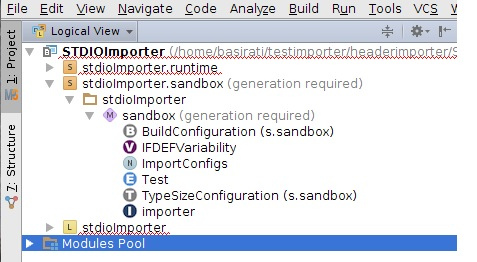
\includegraphics[scale=1]{errscreen.jpg}
\end{figure}

\begin{enumerate}
\item
Right-click on stdioImporter.runtime
\item
Go to Module Properties
\item
In the common tab you need to update the address of bparser.jar file, for doing this you need to follow these steps:
\begin{enumerate}
\item
In section Model Root there are two models. The first is default and the second is a \texttt{java\_classes} model. Bparser.jar file is located under this model (Right now it's red showing that it has some problems, Figure2)
\begin{figure}[ht]
\caption{Missing Jar State}
\centering
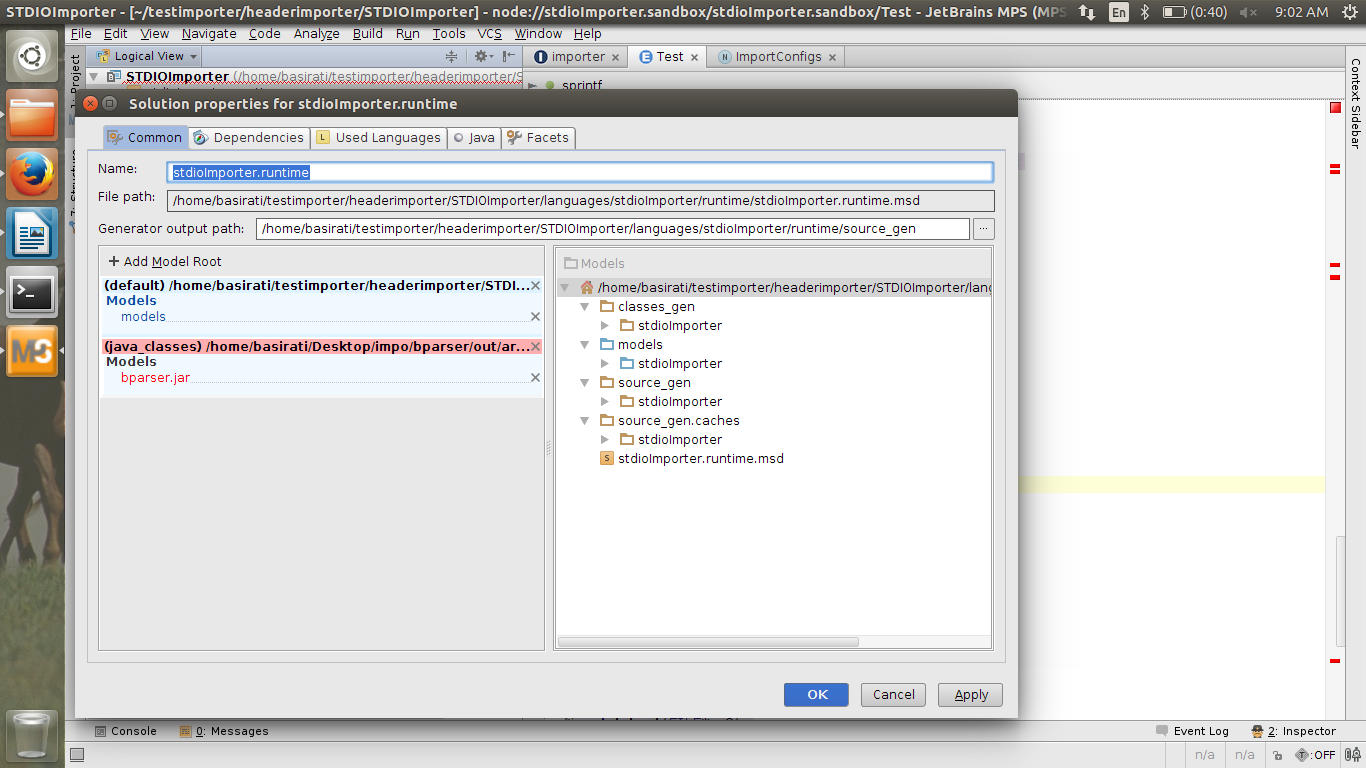
\includegraphics[scale=0.5]{jarmissed.jpg}
\end{figure}
\item
Click on the little cross on the bparser.jar line to delete the old version.
\item
Now click on the \texttt{java\_classes} model line. You will see the model browser window on the right is empty. Right click in the empty area.
\item
Right-click in the right small file browser on the right of the window.
\item
Click on "Change Root Folder".
\item
In the opened file browser select the folder containing the bparser.jar which is: ".../headerimporter/bparser/out/artifacts/\texttt{bparser\_jar}" (Figure 3).
\begin{figure}[h]
\caption{bparser.jar Path Selection}
\centering
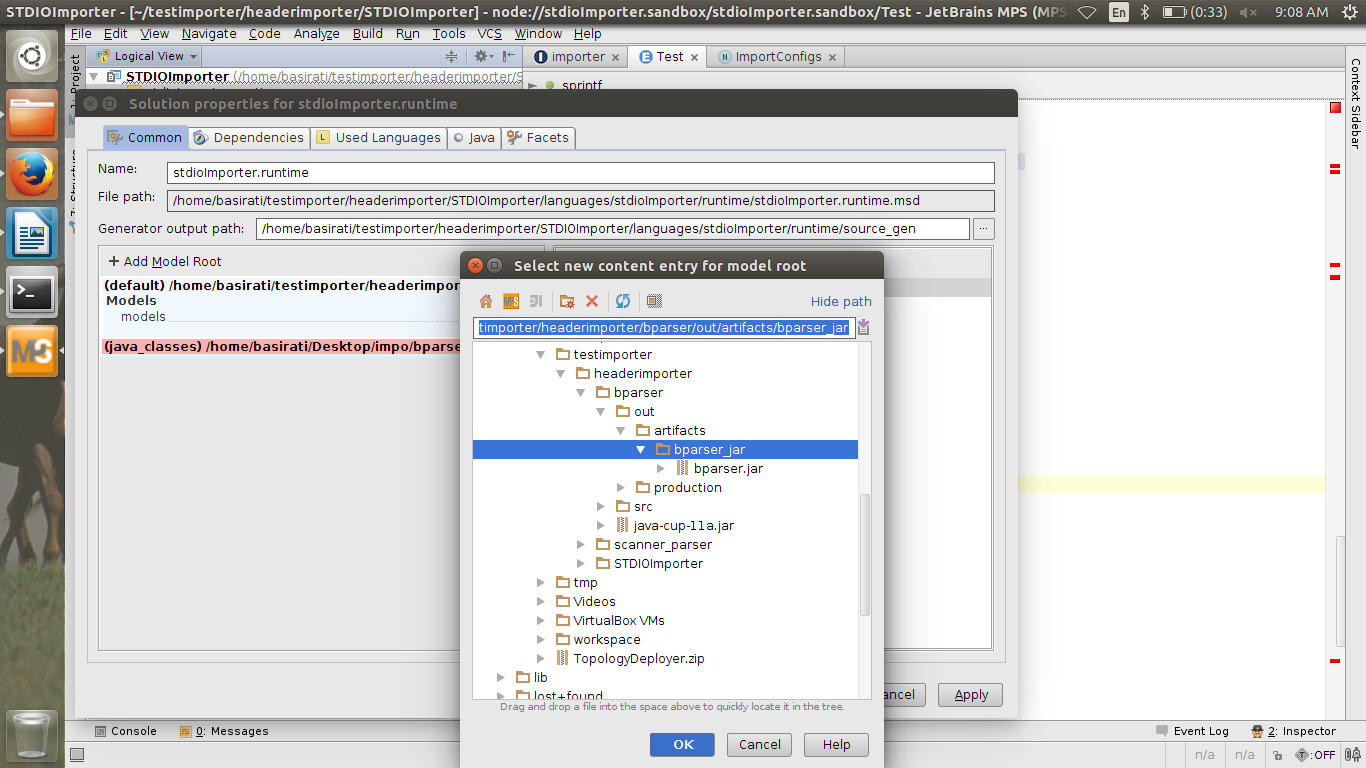
\includegraphics[scale=0.3]{selectpath.jpg}
\end{figure}
\begin{figure}[h]
\caption{Updated Jar State}
\centering
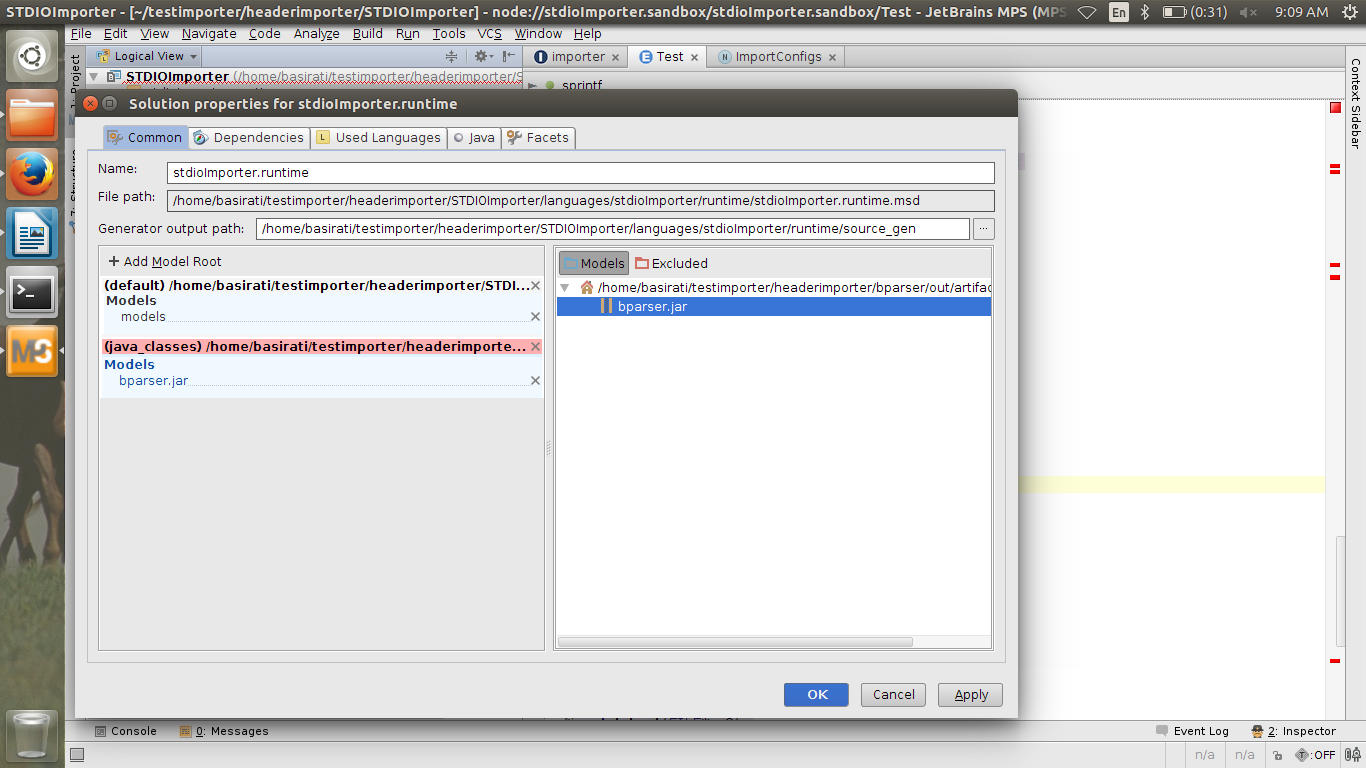
\includegraphics[scale=0.4]{correctjar.jpg}
\end{figure}
\item
Now in the small file browser you should be able to see the bparser.jar file.Right-click on the bparser.jar file and select Models.
\end{enumerate}
\item
Now go to the tab Java. In the libraries section also you need to update the address of bparser.jar. Remove the old bparser.jar by selecting it and clicking on the minus sign on the right of the window (Figure 5).
\begin{figure}[h]
\caption{Java Library Missed Jar State}
\centering
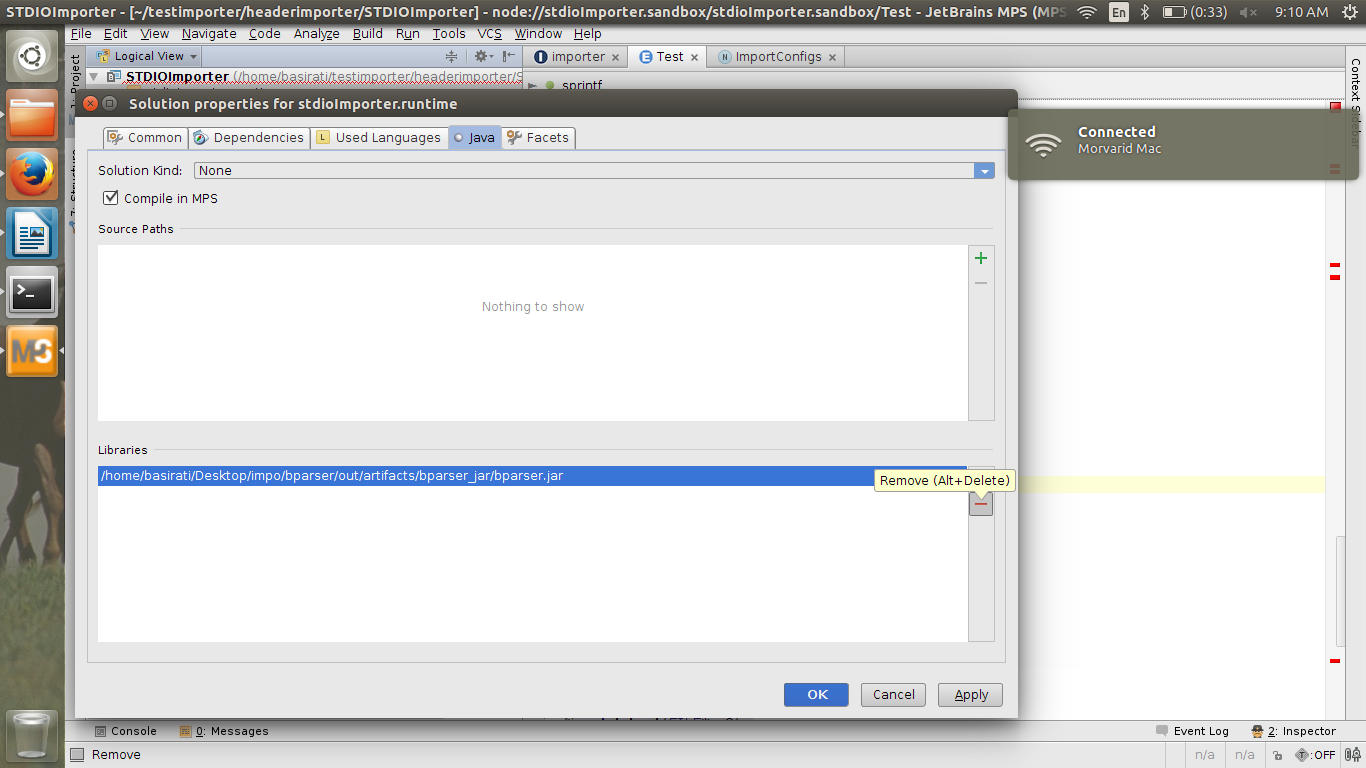
\includegraphics[scale=0.4]{javalibmissed.jpg}
\end{figure}
\item
Now add the new bparser.jar file by clicking on the plus sign and selecting the file in this address:”.../importer-stdio/bparser/out/artifacts/\texttt{bparser\_jar}/bparser.jar”
\item
A dialog will be displayed (Figure 6). Click the OK button.
\begin{figure}[h]
\caption{Opened Dialogue Window}
\centering
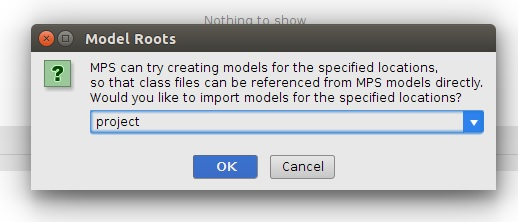
\includegraphics[scale=0.5]{dialog.jpg}
\end{figure}
\item
Now click on apply and the ok buttons.
\item
Now your project should not have any errors.  As the next step you need to rebuild the whole project by right-clicking on the STDIOImporter node and then clicking the rebuild STDIOImporter.
\item
Now the importer is ready to use.
\end{enumerate}
\end{itemize}

\section{How to use the importer?}

The main code of the importer which parse the stdio.h file and import declarations into mbeddr project is located in stdioImporter.runtime module. In stdioImporter language, there are two new concepts added. But you don't need to know or change anything in this section until you want to improve the importer. In the stdioImporter.sandbox module you can use the importer and write your own code. That's where you should start using the importer.

Under the sandbox module you will find a BuildConfiguration, IFDEFVariability, ImportConfigs, Test, TypeSizeConfiguration, and UsingImporter modules.

\begin{itemize}
\item[External Module]
Test module is an external module which means it can hold some declarations and then it can be treated like a c header file in mbeddr. The program code will be written in implementation modules, like UsingImporter module that we have here. So for using declarations in a external module in our implementation module, like including c header files above our c codes, we should import external module above our implementation modules. The main ability of the importer is importing stdio.h header file declarations into an external module, so we can use the declarations in writing our code.

If you open the Test module you will see it's empty. On the top of the page you can see two parts: imports and resources. If a module wants to use another, it should import it in the imports section. For example if you look into UsingImporter module, you will find that it has imported the Test module for using its declarations. In the resources part, we give the address of the header file which the external module holds its declarations. Right now it has set to <stdio.h> that we want to import it.

\item[Import Configs]
ImportConfigs is a new module concept which has been introduced by STDIOImporter. You should have this module to import a header file into an external module. If you look into ImportConfigs module, you will see the line: “import stdio.h into Test form /home/basirati/...”. This line is another new concept introduced by STDIOImporter and it is called ImportConfig. This is the syntax for telling the importer that which header you want to import, where the address of this header file is, and into which external module you want to import. As you can see here, import stdio.h stands for mentioning which header file you want to import, into Test stands for mentioning that we want to import into Test module and from /home/basirati/... stands where is the address of the file we want to import.

First of all, you should update the address in the config line to the address of stdio.h header file that is located in headerimporter folder. Then you can import it into the Test module. For doing this we have an intention. If you keep your cursor on the line you will see a small lamp icon will be appear on the left side of the line. By clicking on the lamp icon you will see a list of intentions available for this concept that one of them will be “Perform Import”. Another way to reach the intentions for a concept is to pressing Alt+Enter keys.

After updating the address of the header file, do the “Perform Import” intention. After performing you will find all stdio.h declarations in the Test external module. You probably will see some error on some lines, but don't worry, it's OK. Importing ifdefs caused these errors and there will be no problem at the build time.

\item[mbeddr Variability]
For importing the ifdefs we have implemented them by the mbeddr concept, “variability”. Mbeddr introduces variability concept that enables writing a code with different features and selecting some of the features to be built at the end, based on what we want to do. In mbeddr we have static and runtime variability. For implementing ifdefs we used static variability. For more information about variability see the mbeddr guidelines and this paper: http://mbeddr.com/files/tomassettiratiu-extractingvariabilityfromcandliftingittombeddr.pdf.

\item[Importing ifdef]
Every ifdef or ifndef is a feature, it means when we want to build the project we can say which feature it should use. IFDEFVariabilty module introduces the ifdefs and ifndefs as features to the mbeddr project. If you open it, you can see it has two sections, "feature model" IFDEFS, and "configuration model" allconfigurations configures IFDEFS. As you can see, the name of features in our feature model is as the same as the names of ifdefs variables. For example if we had the line ifdef FILE in the stdio.h header file, here we have the feature FILE.

In configuration model section you can see that some of features in the feature model has been mentioned here too. It means by selecting this configuration model, you will enable its features at the build time. You can add your own configuration model and customizing the features, here ifdefs, for building your own project.

Features can have child features that in our context it means we had some ifdefs into each other. The else part of a ifdef has been implemented by selecting a logical not of a feature, e.g. {!FILE}.

As you can see above the Test module after performing the import, there is a Variant Selection that tells which features has been configured for this module by selecting the configuraiton model. MPS provides a feature that can help you understand better about the variability concept. On the menu bar you can find the Code section. Under the Code section there is Projection Mode. Here you can select between “Compact Product Line”, “Detailed Product Line”, and “Selected Variant”. You will see by selecting the “Selected Variant”, you can only see declarations in Test module that has a feature in selected configuration model.

\item[Build Variability Configuration]
Now you can go to UsingImporter module and write some code that uses the declarations in Test module.

The last step for using the importer is to set variability configurations for building the project. For this job, you should go to the BuildConfiguration module. In the Configuration Items section you should tell the mbeddr which configuration model you wants to be build. For doing this you should add a line like the figure 7. Remember that you should update this line every time you perform import or change the IFDEFVariability module. In the Binaries section, you need to add the external module, in our example the Test module, too.

Now you can build your project and use all declarations in the stdio.h header easily.

\begin{figure}[ht]
\caption{Opened Dialogue Window}
\centering
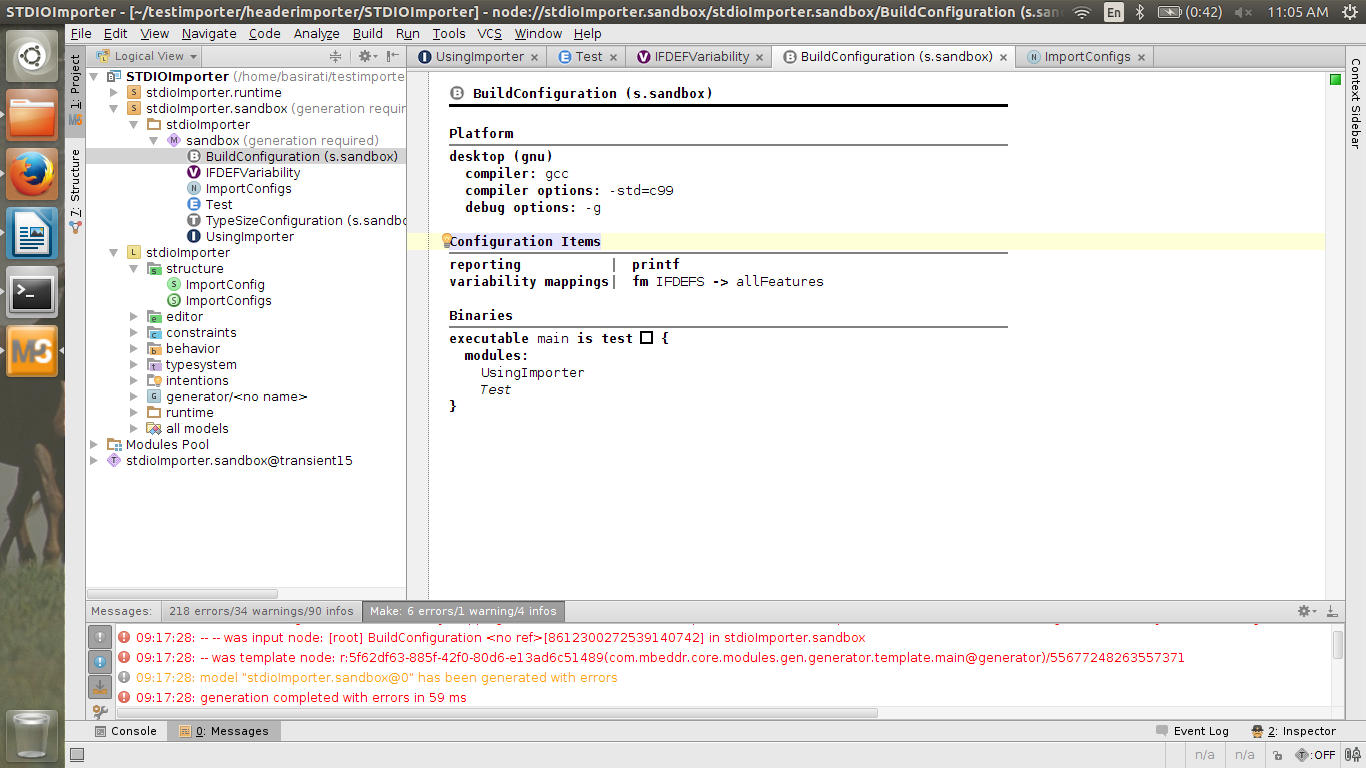
\includegraphics[scale=0.3]{buildsett.jpg}
\end{figure}

\end{itemize}




















\end{document}
